\chapter{Návrh a implementace rozšíření}
Rozšíření bude, jak již bylo nastíněno výše, implementováno v jazyce Typescript. 
K vytvoření rozšíření samotného je potřeba Node.js a Git. Poté je vyžadována instalace programu "Yeoman" "VS Code Extension Generator".

\section{Error Listener}
Slouží k zachytávní syntaktických chyb v kódu, čili chyb, které jsou v rozporu z pravidly gramatiky. Rozšíření chyby vypisuje do konzole, jak jsme ve VS Code zvyklí. Součástí zprávy jsou:
\begin{enumerate}
\item řádek, na kterém se chyba nachází
\item pozice na řádku
\item popis chyby
\end{enumerate}

\section{Modul Toybox}
Tento modul (modul = namespace) obsahuje všechny potřebné třídy, se kterými v Monkey C můžeme pracovat.

\section{Zvýraznění kódu}

Zvýraznění, nebo-li obarvení klíčových slov kódu je realizováno pomocí JSON souboru, jenž pomocí regulárních výrazů v textu vyhledává příslušná slova a ty poté obarvuje.
\\
\begin{figure}
	\centering
	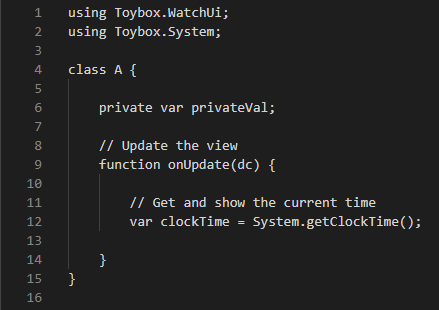
\includegraphics[]{images/uncolored_code}
	\caption{ukázka neobarveného kódu v MonkeyC}
	\label{img:uncolored_code}
\end{figure}

\begin{figure}
	\centering
	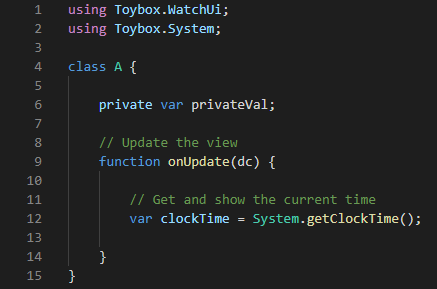
\includegraphics[]{images/colored_code}
	\caption{ukázka obarvení kódu v MonkeyC} 
	\label{img:colored_code}
\end{figure}
	
Hned na první pohled je zřejmé, že obarvení poskytuje uživateli větší přehled a orientaci v kódu, jak je vidět na obrázku \ref{img:colored_code}


\section{Automatické doplňování a našeptávání kódu}

Hlavním aktérem při našeptávání vhodných částí kódu je "antlr4-c3 The ANTLR4 Code Completion Core".

Jedná se o "stroj" sloužící k dokončování gramatického agnostického kódu pro analyzátory založené na ANTLR4. Engine c3 je schopen poskytnout kandidáty na doplnění kódu, kteří jsou užiteční pro editory s analyzátory generovanými ANTLR, nezávisle na skutečném jazyku / gramatice použité pro generování.

Původní implementace je poskytována jako "node module" a je psána v jazyce Typescript.

Pro zobrazení možných symbolů ve zdrojovém kódu zjevně potřebujete zdroj pro všechny dostupné symboly na dané pozici. Jejich poskytnutí je obvykle úkolem tabulky symbolů. Jeho obsah lze odvodit z vašeho aktuálního zdrojového kódu (pomocí analyzátoru + analyzátoru Listeneru). Statičtější části (například runtime funkce) lze načíst z disku nebo poskytnout pevně zakódovaný seznam atd. Tabulka symbolů pak může odpovědět na vaši otázku ohledně všech symbolů daného typu, které jsou viditelné z dané pozice. Pozice obvykle odpovídá konkrétnímu symbolu v tabulce symbolů a struktura pak umožňuje snadno získat viditelné symboly. Engine c3 je dodáván s malou implementací tabulky symbolů, která však není pro použití knihovny povinná, ale poskytuje snadný start, pokud již nemáte vlastní třídu tabulek symbolů.

Zatímco tabulka symbolů poskytuje symboly daného typu, musíme zjistit, který typ je ve skutečnosti vyžadován. To je úkol enginu c3. V nejjednodušším nastavení vrátí pouze klíčová slova (a další symboly lexerů), která jsou povolena gramatikou pro danou pozici (což je samozřejmě stejná pozice, která se používá k nalezení kontextu pro vyhledávání symbolů ve vaší tabulce symbolů). Klíčová slova jsou pevná sada slov (nebo sekvencí slov), která se obvykle nenachází v tabulce symbolů. Skutečné textové řetězce můžete získat přímo ze slovníku analyzátoru. C3 za ně vrací pouze lexerové tokeny.


\begin{figure}[h!]
	\centering
	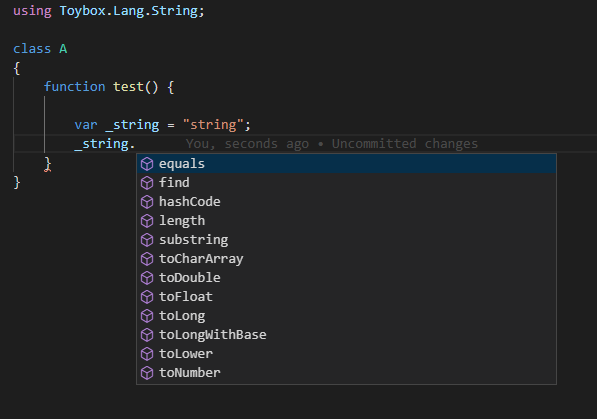
\includegraphics{images/autocomplete_example}
	\caption{ukázka automatického našeptávání kódu na proměnné typy string}
	\label{img:autocomplete_example}
\end{figure}

\section{komentáře}
Základním prvkem pro práci s komentáři je třída ToyBox. Jedná se o stěžejní modul (Modul v Monkey C je ekvivalentem Namespace např v. C Sharp), ve kterém jsou obsaženy všechny třídy, funkce, proměnné, se kterými MonkeyC pracuje. Toybox, jako takový není nikde oficiálně dostupný, tudíž bylo nutné tento hlavní modul vygenerovat. Zdrojem pro generování bylo Connect IQ SDK.

\begin{figure}
	\centering
	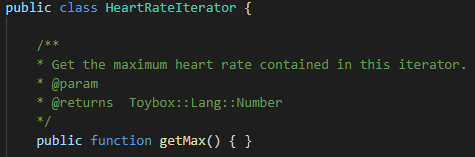
\includegraphics{images/comments}
	\caption{komentář nad funkcí obsahující stručný popis, parametry funkce a návratový typ}
	\label{img:comments}
\end{figure}

\section{nedostatky rozšíření}
Při implementaci automatického našeptávání byl detekován problém, kvůli kterému není možné provést volání více funkcí po sobě na jednom řádku. Uveďme si příklad, kdy máme proměnnou typu \textbf{String}, v níž je uloženo číslo. Hodnotu v této proměnné budeme chtít převést na typ Integer, čili zavolat metodu \textit{toNumber()}, a poté bezprostředně po volání \textit{toNumber()} zavolat další metodu. Zde nastává problém, kdy rozšíření, jako další vstup neočekává možné volání funkce \ref{img:autocomplete_errormessage}. Jádrem tohoto problému je, že poskytnutá bezkontextová gramatika popisující jazyk není stoprocentně přesná. A právě kvůli těmto "nepřesnostem" je možné při implementaci narazit na podobné komplikace. V průběhu vývoje zatím nebyly registrovány další problémy způsobené gramatikou.

\begin{figure}
	\centering
	
\includegraphics[scale=1]{images/autocomplete_error}
	\caption{nedostatek rozšíření}
	\label{img:autocomplete_error}
\end{figure}

\begin{figure}
	\centering
	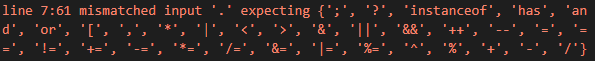
\includegraphics[scale=0.8]{images/autocomplete_errormessage}
	\caption{chybová hláška z error listeneru}
	\label{img:autocomplete_errormessage}
\end{figure}
\endinput